%!TEX root = ../thesis.tex
\define{\imgpath}{french/img}

\chapter*{Résumé substantiel}
\label{chapter:frecnhresume}
\minitoc

Cette thèse s'intéresse à un problème logique dont les enjeux théorique et pratique sont multiples. Ce problème, dans sa forme simple, peut-être présenté ainsi: Imaginez que vous êtes dans un labyrinthe, dont vous connaissez toutes les routes menant à chacune des portes de sortie. Derrière l'une de ces portes se trouve un trésor; mais vous n'avez le droit d'ouvrir qu'une seule porte. Un vieil homme habitant le labyrinthe connait la bonne sortie et se propose alors de vous aider à l'identifier. Pour cela, il vous indiquera la direction à prendre à chaque intersection. Malheureusement, cet homme ne parle pas votre langue, ainsi les mots qu'il utilise pour dire ``droite'' ou ``gauche'' vous sont inconnu. Est-il possible de trouver le trésors et de comprendre l'association entre les mots du vieil homme et leurs significations ?

Ce problème, bien qu'en apparence abstrait, est relié à des problématiques concrètes dans le domaine de l'interaction homme-machine que nous présentons aux chapitres~\ref{chapter:introduction} et \ref{chapter:relatedwork}. En effet, si nous renversons les rôles: un utilisateur, prenant la place du vieil homme, souhaite guider un robot vers la bonne sortie du labyrinthe. Ce robot ne sait donc pas en avance quel est la bonne sortie mais il sait où se trouvent chacune des portes et comment s'y rendre. Imaginons maintenant que ce robot ne comprenne pas a priori le langage de l'humain; en effet il est très difficile de construire un robot à même de comprendre parfaitement chaque langue, accent, et préférence de tout un chacun. Il faudra alors que le robot apprenne l'association entre les mots de l'utilisateur et leur sens, tout en réalisant la tâche que l'humain lui indique (e.g. trouver la bonne porte). Ce problème n'est pas simple car pour comprendre le sens des signaux il faudrait connaitre la tâche, et pour connaître la tâche il faudrait connaitre le sens des signaux.

Il s'agit donc, pour un labyrinthe donné, de trouver la suite d'action permettant de collecter suffisamment d'information de la part de l'humain pour comprendre à la fois le sens de ses mots et la porte derrière laquelle se cache le trésor. Cela dépend donc de la configuration du labyrinthe et de l'historique complet de l'interaction entre les deux protagonistes.

Dans cette thèse nous présentons une solution à ce problème. Pour cela nous faisons d’abord l'hypothèse qu'un nombre fini de tâche est défini et connu de l'homme et de la machine, i.e. un nombre fini de portes existe. Nous supposons également que le robot dispose d'un modèle de la logique de l'utilisateur et est donc capable de faire le raisonnement suivant: Si l'humain veut que j'aille vers la Porte $1$ alors lorsque je suis à l'intersection $I$, il devrait logiquement me dire d'aller dans la direction $D$. Noter que cette phrase commence par une supposition sur la tâche, qui n'est en aucun cas connu à l'avance. Ainsi, le robot étant équipé de plusieurs hypothèses (Porte $1$, $2$, $3$, ..), lorsqu'il se trouve à l'intersection $I$, l'utilisateur prononce un mot (e.g. "wadibou"), dont autant d'interprétations sont faite que d'hypothèses sur la tâche.

Notre hypothèse sous-jacente est que l'utilisateur est logique et cohérent tout au long de l'interaction, utilisant ainsi toujours le même mot pour dire la même chose. Il nous faut donc tenir compte de tout l'historique de l'interaction pour analyser quels mots auraient été utilisés pour dire quoi selon chaque hypothèse de tâche. Nous comprenons ainsi que, sous certaine conditions qui sont explicitées au chapitre \ref{chapter:lfui}, il est possible d'éliminer toutes les hypothèses générant des interprétations incohérentes du sens des signaux. L'unique hypothèse restante nous informera donc à la fois de la bonne tâche, i.e. la bonne porte à ouvrir, mais aussi de la bonne association entre les mots de l'utilisateur et les sens qui y sont associés, i.e. du langage de l'utilisateur.

Une autre façon de décrire ce travail est de parler d'auto-calibration. En effet, en s'adaptant à l'utilisateur pendant l'interaction, notre algorithme ne fait aucun apriori sur le sens des signaux qu'il reçoit. Cela revient bien à créer des interfaces ne nécessitant pas de phase de calibration car la machine peut s'adapter, automatiquement et pendant l'interaction, à différentes personnes qui ne parlent pas la même langage ou qui n'utilisent pas les mêmes mots pour dire la même chose. Cela veut aussi dire qu'il est facile d'étendre notre approche à d’autres modalités d'interaction (e.g. gestes, expression faciales, onde cérébrales) et d'autre domaine d'applications.

% Une personne au capacités de communication réduite doit utiliser une machine pour communiquer avec le monde extérieur, il doit donc pouvoir la commander.

Remplaçons par exemple le problème du labyrinthe par une tâche plus concrète, plus utile. Prenons donc l'exemple d'une personne aux capacités de communication réduite avec le monde extérieur. Ne pouvant utiliser par exemple que de fragile clignement des yeux ou aillant recours à l'enregistrement de leurs ondes cérébrales (EEG). Il devient alors difficile, voir même impossible de savoir à l'avance les intentions de communications de ces personnes. Il est donc primordial de disposer de machine qui sont à même de s'adapter automatiquement à chaque personne. Ainsi il n'est pas surprenant de voir que c'est la communauté de l'interaction cerveau-machine (BCI) qui s'est intéressée le plus au problème de l'auto-calibration. En effet, à l'opposé des modes d'interaction classique, telle que la parole, les gestes ou les expressions faciales, nous avons très peu d'apriori sur l'utilisation des signaux du cerveau.

\subsection*{Résultats}

Notre approche est donc très générique et permet à un humain de commencer à interagir avec une machine afin de résoudre une tache séquentielle sans que la machine ne comprenne à l'avance les signaux de communications de l'utilisateur.

Nous appliquons nos algorithmes d'auto-calibration à deux exemples typique de l'interaction homme-robot et de l'interaction cerveau-machine: une tâche d'organisation d'une série d'objets selon les préférences de l'utilisateur qui guide le robot par la voix (chapitre~\ref{chapter:lfui}, voir figure~\ref{fig:setupfrench} - gauche), et une tâche de déplacement sur une grille guidé par les signaux cérébraux (EEG) de l'utilisateur (chapitre~\ref{chapter:bci}, voir figure~\ref{fig:setupfrench} - droite).

\begin{figure}[!htbp]
  \centering
  \includegraphics[width=0.49\columnwidth]{chapters/lfui/img/setup.png}
  \includegraphics[width=0.49\columnwidth]{\visualspdf/onlineXP/setup.pdf}
  \caption{Illustration des deux setups expérimentaux tangible utilisé dans ce travail. Gauche: Le bras robotique pour la tâche d'organisation de trois cubes. Droite: L'interface cerveau machine composée d'un casque avec ces électrodes et d'un écran affichant les informations relatives à la tache.}
  \label{fig:setupfrench}
\end{figure}

Bien que les expériences du chapitre~\ref{chapter:lfui} sont fondatrice, pour ce bref résumé nous préférons nous concentrer sur les expériences BCI qui présentent un aspect plus appliqué car testé sur de vrai sujets en temps réel et sur une tâche d'actualité pour les interfaces cerveau-machine.

Au chapitre \ref{chapter:bci}, nous présentons donc l'application principale de ce travail aux interfaces cerveau-machine. Ce genre d'interface permet aux personnes à fort handicap d'interagir avec le monde extérieur par le biais de leur cerveau. Plus précisément, nous pouvons enregistrer des variations de potentiel à la surface de leur cerveau. Ces ondes ont des propriétés différentes en fonction de l'activité mentale du sujet et il est possible de différentier différentes activités motrices ou même des signaux d'erreur de type oui/non. Le problème de ces systèmes est qu'ils ne sont pas universels et doivent être adapté à chaque utilisateur. Cette adaptation est faite par le biais d'une phase de calibration, souvent ennuyeuse, ou l'utilisateur doit répéter plusieurs centaines de fois les mêmes actions mentales et durant laquelle le système est inutilisable; de plus nécessitant l'intervention d'une personne extérieur. Non seulement cette phase de calibration est ennuyeuse et rébarbative mais elle doit  être effectué régulièrement car les signaux varient de jour en jour ou car la position du casque change.

% Enfin au chapitre \ref{chapter:bci}, nous présentons les résultats d'expériences réel dans le cadre de l'interaction cerveau-machine.

L'utilisation d'algorithmes d'auto-calibration permettrait donc un plus grande flexibilité et aisance d'utilisation de ces technologies et permettrait de les utiliser chez soi sans la supervision d'un spécialiste.

Dans cette thèse nous présentons donc des expériences ou des sujets humains ont pour tâche de guider un agent dans un labyrinthe en lui indiquant si ces actions sont ``correcte''  ou ``incorrecte'' vis a vis de l'objectif cible défini simplement en pensant à ``correcte'' ou ``incorrect'' dans leur esprit. Les ``pensées'' de l'utilisateur sont mesuré par le biais d'électrode au contact de son cerveau. Le setup expérimental est celui présenté sur la figure~\ref{fig:setupfrench} (droite).

La figure~\ref{fig:sequencefrench} présente le résultat principale de cette thèse. Elle compare la différence entre un algorithme nécessitant une phase de calibration et les algorithmes d'auto-calibration développé dans cette thèse.  Ce sont des résultats de simulation avec des données EEG réelle. Notre algorithme (figure~\ref{fig:sequencefrench} - haut) permet de résoudre une première tache en seulement 85 itérations, bien avant que la phase de calibration ne soit complète (400 itérations étant une période typique de calibration pour ce genre de système).
Enfin notre méthode résout une dizaine de tache en 400 itérations, soit avant qu'un système traditionnel ne soit opérationnel.

\begin{figure}[!htbp]
\centering
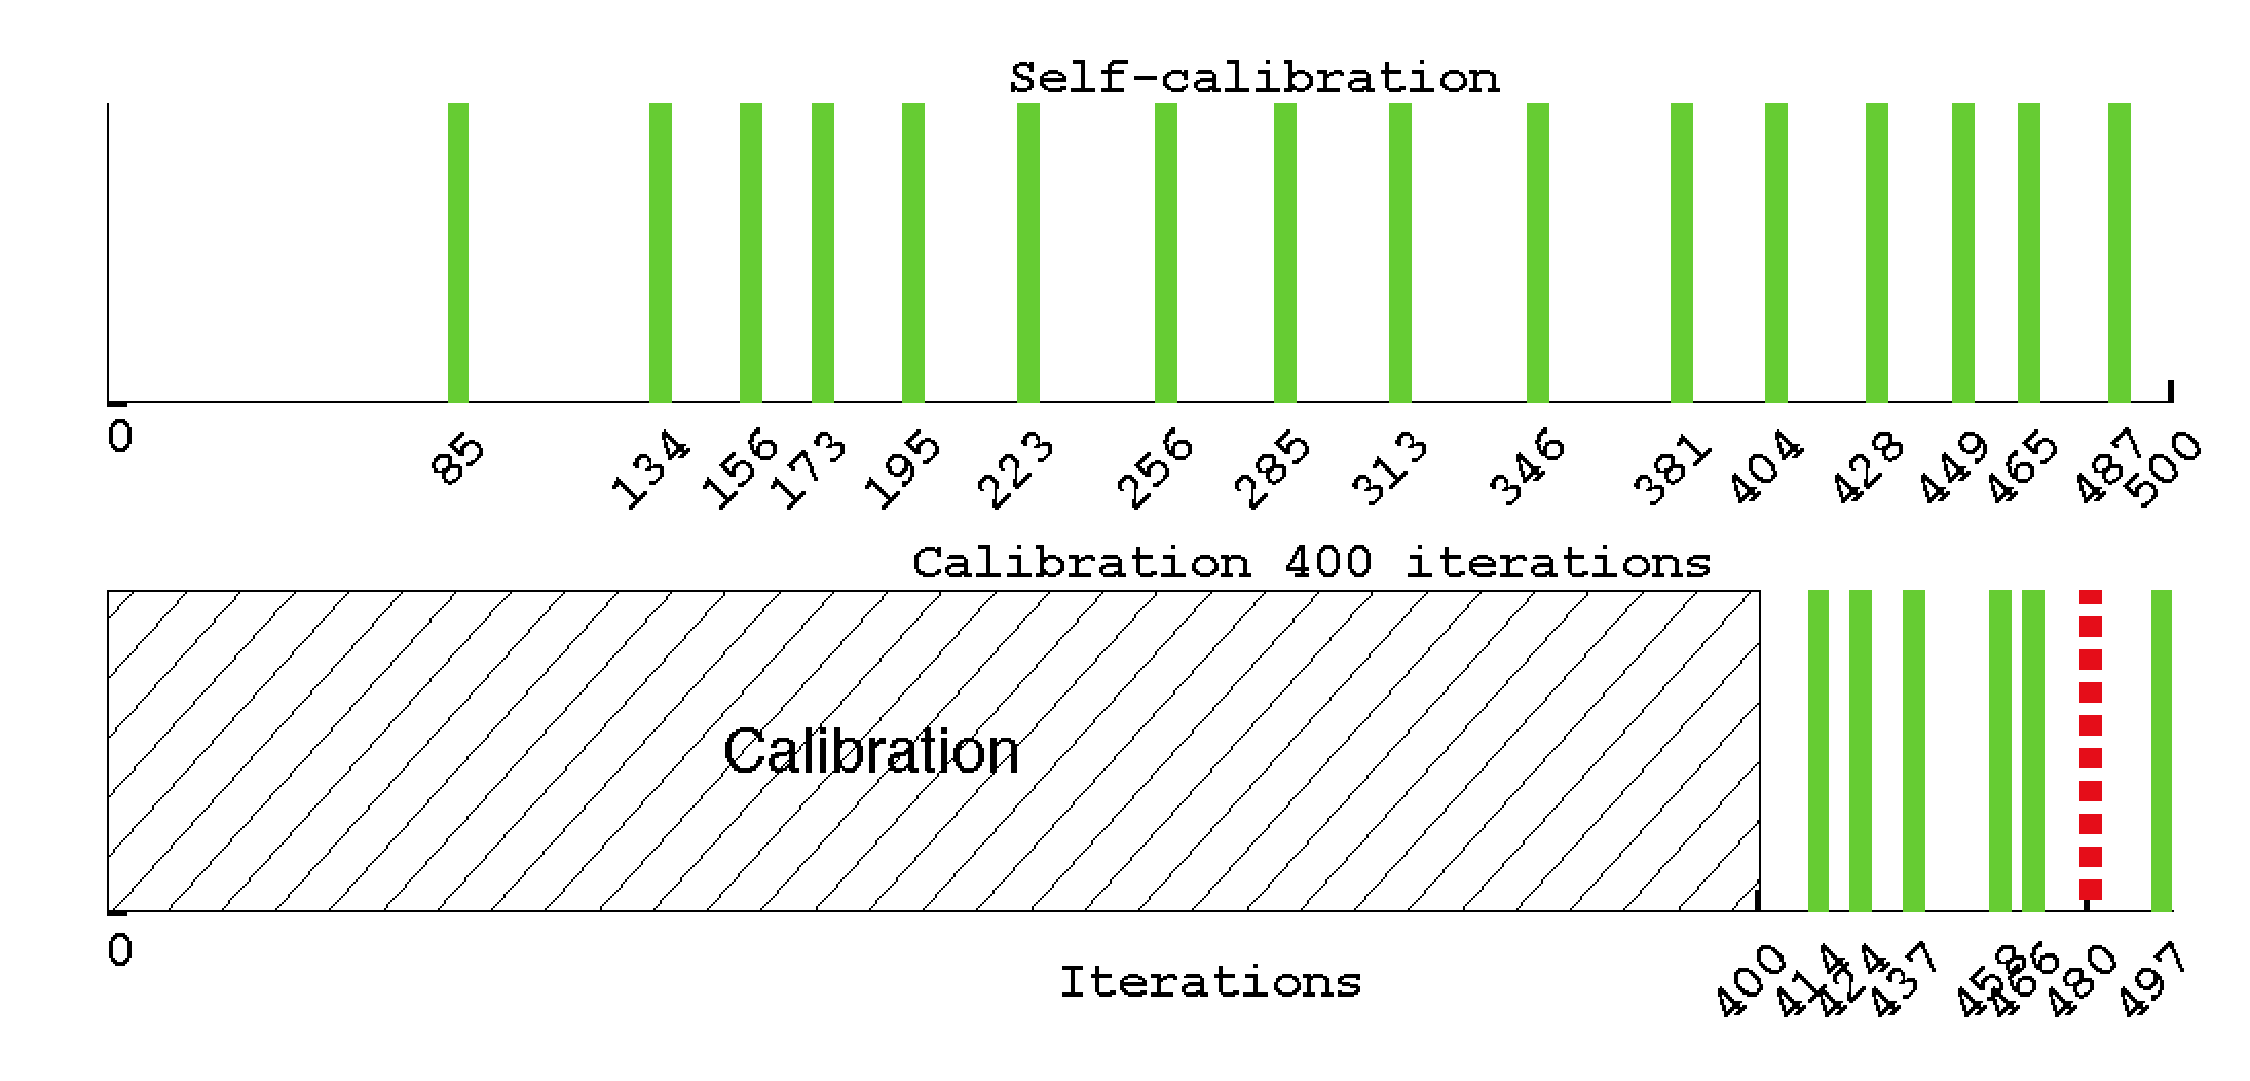
\includegraphics[width=\sequencesize\columnwidth]{\imgpath/plot_the_aaai_sequence.eps}
\caption{Nombre de tâche résolue dans le temps avec des données EEG. L'algorithme d'auto-calibration (haut) est comparé aux méthodes nécessitant une phase de calibration (bas, ici 400 itérations de calibration Le barres verte et rouge représente respectivement les bonnes et les mauvaise exécutions de la tâche par la machine. La méthode d’auto calibration proposée dans cette thèse permet de compléter une première tache plus rapidement, sans pour autant faire d'erreur.}
\label{fig:sequencefrench}
\end{figure}

Les même expériences on été testé avec des utilisateurs réel. Leur résultats confirme ceux de simulation et sont présenté au chapitre \ref{chapter:bci} ainsi qu'au chapitre \ref{chapter:limitations:overlap}. Nos résultats démontrent expérimentalement que notre approche est fonctionnelle et permet une utilisation pratique de l'interface plus rapidement. De plus notre système ne nécessite pas la présence d'une personne extérieure pour calibrer le système et est donc un candidat potentiel pour amener l'utilisation des interfaces cerveau machine dans les maisons.

\subsection*{Planification des actions}

Un autre résultat important de cette thèse est le planning est également différent des algorithmes précédemment développés. En effet une couche d'incertitude supplémentaire est présente, le sens des signaux est inconnu et nous disposons d'une multitude de candidat possible. Il faut donc inclure cette incertitude dans la mesure d'incertitude globale permettant de naviguer plus efficacement dans le monde. Afin de collecter des signaux varié. Les résultats présente au chapitre montre que notre méthode de planification des actions améliore significativement le temps nécessaire à l'identification de la tâche mais aussi à l'établissement du modèle de langage de l'utilisateur.
\ref{chapter:planning}

\subsubsection*{Extensions}

\ref{chapter:limitations:continousstate}
\ref{chapter:limitations:continuoushypothesis}
\ref{chapter:limitations:framehypothesis}
\ref{chapter:limitations:proof}


Au chapitre~\ref{chapter:limitations}, nous abordons et proposons des solutions à de multiples limitations de l'approche présentée dans cette thèse. Nous montrons d'abord qu'il est possible d'utiliser le système dans des espaces continue: premièrement pour un état continue du système mais sur un ensemble infini d'hypothèse sur la tâche. Par la suite, nous montrons que la connaissance a priori du protocole d'interaction n'est pas une limitation forte et que notre système peut détecter le protocole par l'interaction pratique avec l'utilisateur.

Etrangement, cette thèse ne traite pas directement du problème simple, symbolique, mais s'intéresse d'abord à une représentation non-symbolique des signaux de communications. Ceci dans un but applicatif à courts termes auquel de fastidieuses preuves mathématiques dans des domaines trop simplifiés n’auraient laissé guère de temps à l'expérimentation. Ainsi la formulation simple du labyrinthe présentée au début de ce résumé n'est adressé que dans la toute dernière section de cette thèse par une preuve de la validité de notre solution pour le cas de signaux de communication symbolique et sous de forte contrainte de l'environnement. Ce dernier développement montre que ce genre de problème peut-être modélisé mathématiquement et ouvre la voie de prochaine exploration plus théorique de ce problème. Permettant peut-être de trouver des  garantie plus grande sur la convergence et les performance de nos algorithmes. Bien que ce genre de preuve semble encore très limité pour l'interaction pratique de par la nature imprévisible du comportement humain.

% Finalement, nous démontrons mathématiquement sur un exemple simplifié et sous certaines conditions que notre méthode est garantie d'identifier la bonne hypothèse.

\subsection*{Expèrience humain-humain}

Une autre contribution de cette thèse et la mise en place d'un protocole expérimental pour analyser le comportement de deux humain mis dans la situation que doivent résoudre nos algorithmes (chapitre~\ref{chapter:humanexperiment}). Dans cette expérience deux humains doivent collaborer à l'exécution d'une tâche de construction. Ils ne peuvent interagir que par le biais d'une interface dont le sens des signaux transmis est inconnu et indéfini au départ pour les deux parties.

Il sera intéressant de voir la dynamique de construction d'un langage commun entre les deux participants. Langage qui n'était pas prévu au début de l'interaction s'établi de tel sorte qu'une personne extérieure à l'expérience ne pourra alors pas comprendre ce qui ce passe en observant le résultat final de l'interaction.

\subsection*{Conclusion}

La vision développée dans cette thèse est qu'il est possible pour une machine d'interagir avec un humain sans comprendre a priori la façon dont l'utilisateur communique l'information. Plus concrètement notre système n'a pas d'apriori sur le sens des signaux reçu et construit son modèle durant l'interaction pratique avec l'utilisateur sans jamais avoir accès a une source sûre d'information. Cela sera, nous l'espérons, le fruit de nombreux travaux futur.

Au delà du challenge technique de l'auto-calibration, des questions d'utilisation pratique et d'acceptabilité éclosent et sont présentées au chapitre~\ref{chapter:limitations:userstudies}. Parmi elles, la plus importante à tester en condition réelle est: Comment les utilisateurs vont réagir au fait que la machine, le robot, ne soit pas immédiatement réactif à ces ordres mais doivent apprendre le sens des signaux pendant l'interaction? En effet, même si nos algorithmes apportent une plus grande flexibilité d'interaction, ils ne permettent pas à l'utilisateur une fonctionnalité parfaite et immédiate du système qui doit en effet apprendre de l'interaction. Cette phase d'apprentissage pourrait être perçus comme une inopérabilité du système et par conséquent impacter l'intérêt et l'utilisabilité réelle de notre système.\\

\noindent {\large\textbf{Mots-clés:}} Auto-Calibration, Apprentissage par interaction, Interaction Humain-Robot, Interface Cerveau-Machine, Interaction Intuitive et Adaptative, Robotique, Acquisition de Symbole, Apprentissage Actif, Calibration.\\

Ce travail a été financé par INRIA, le Conseil Régional d'Aquitaine et la bourse ERC EXPLORERS 24007.
